\section{Measurable Functions}

  So far, we have defined measurable sets, constructed the Lebesgue measure, and shown that Lebesgue measurable sets can be approximated by nice open sets. Now, let's talk about measurable functions. Just like for measurable sets, there is a general sense in which we can define them and there is the more ``Euclidean'' way of defining them. 

  \begin{definition}[Measurable Function]
    Given a measurable space $(X, \mathcal{A})$, $f: (X, \mathcal{A}) \longrightarrow \mathbb{R}$ is \textbf{measurable} if 
    \begin{equation}
      f^{-1}(A) \in \mathcal{A} \text{ for all } A \text{ open}
    \end{equation}
    Note that measurable functions are always defined on measurable sets, so we don't have to state that its domain is always measurable. 
  \end{definition}

  \begin{theorem}[Measurable Functions on Real Line]
    Let $f: E \subset \mathbb{R} \to \mathbb{R} \cup \{ \pm \infty\}$ and $E$ be measurable. Then, TFAE 
    \begin{enumerate} 
      \item $\forall c \in \mathbb{R}$, $\{x \in E \mid f(x) > c\}$ is measurable. 
      \item $\forall c \in \mathbb{R}$, $\{x \in E \mid f(x) \geq c\}$ is measurable. 
      \item $\forall c \in \mathbb{R}$, $\{x \in E \mid f(x) < c\}$ is measurable. 
      \item $\forall c \in \mathbb{R}$, $\{x \in E \mid f(x) \leq c\}$ is measurable. 
      \item $f$ is Lebesgue measurable. 
    \end{enumerate}
    Furthermore, if any of these hold, then also $\{x \in E \mid f(x) = c \}$ is measurable for all $c$ (but not the converse!). 
  \end{theorem} 
  \begin{proof}
    We know that $(1) \iff (4)$ and $(2) \iff (3)$ by taking complements. We prove $(1) \iff (2)$. 
    \begin{enumerate}
      \item $(1) \implies (2)$. 
      \begin{equation}
        \{x \in E \mid f(x) \geq c \} = \bigcap_{k=1}^\infty \{x \in E \mid f(x) > c - \frac{1}{k} \}
      \end{equation}

      \item $(2) \implies (1)$. 
      \begin{equation}
        \{ x \in E \mid f(x) > c\} = \bigcup_{k=1}^\infty \{x \in E \mid f(x) \geq c + \frac{1}{k} \}
      \end{equation}
    \end{enumerate}

    For $(5)$, we know that
    \begin{enumerate}
      \item $(5) \implies (1)$ is trivial, since open intervals are open sets. 
      \item $(1) \implies (5)$. Any open set is a countable union of disjoint open intervals, and so let 
      \begin{equation}
        U = \bigcup_{k=1}^\infty I_k, \qquad I_k = (a_k, b_k) = \underbrace{(-\infty, b_k)}_{B_k} \cap \underbrace{(a_k, +\infty)}_{A_k}
      \end{equation} 
      Therefore, 
      \begin{equation}
        f^{-1} (U) = \bigcup_{k=1}^\infty f^{-1} (B_k \cap A_k) = \bigcup_{k=1}^\infty \{f^{-1} (B_k) \cap f^{-1} (A_k) \}
      \end{equation}
      which is measurable since countable union/intersections are measurable (by definition of $\sigma$-algebra). 
    \end{enumerate}

    For the final implication, we can use $(2)$ and $(4)$ to get 
    \begin{equation}
      \{x \in E \mid f(x) = c\} = \{x \in E \mid f(x) \leq c \} \cup \{x \in E \mid f(x) \geq c \}
    \end{equation}
  \end{proof} 

  The first question is how you would relate this to continuity. 

  \begin{theorem}[Continuous Functions are Measurable]
    If $f: X \to \mathbb{R}$ is continuous, then it is measurable. 
  \end{theorem}
  \begin{proof}
    If $f$ is continuous, then $f^{-1} (O) = U \cap X$ for every open $O$ with open $U$. 
  \end{proof}

  \begin{theorem}[Monotonic Functions are Measurable] 
    Let $I$ be an interval. If $f: I \subset \mathbb{R}$ is monotone, then $f$ is measurable.
  \end{theorem}
  \begin{proof}
    You can probably see that it is more advantageous to prove using the definition of measurability using rays. We wish to show that for all $c$, $E_c \coloneqq \{x \in I \mid f(x) > c\}$ is measurable. We wish to show that $E_c$ is an interval, though there seems to be some complications with potential discontinuities. 

    Therefore, we use an equivalent definition of an interval: $I$ is an interval if for every $x, y \in I$, $x < t < y \implies t \in I$. Therefore, we can see that if $x, y \in E_c$, then $f(x) > c, f(y) > c$. Therefore, if $t$ is in between them, $f(t) > f(\min\{x, y\}) > c$, and so $t \in E_c$. Since intervals are measurable, we are done. 
  \end{proof}

  There is also some notion of robustness. 

  \begin{theorem}[Function Difference on Measure 0 Set Doesn't Affect Measurability]
    Suppose $f: E \subset \mathbb{R} \to \mathbb{R} \cup \{\pm \infty\}$ with $E$ measurable, and let $g$ be some other function. If $f$ is measurable on $E$ and $g(x) = f(x)$ a.e. for $x \in E$, then $g$ is measurable on $E$. 
  \end{theorem}
  \begin{proof}
    We wish to show that for any open $O \subset \mathbb{R}$, $g^{-1} (O)$ is measurable. We might start with Carathéodory and try to show that for all $A \subset E$, 
    \begin{equation}
      m^\ast(A) = m^\ast (A \cap g^{-1}(O)) + m^\ast (A \cap g^{-1}(O)^c)
    \end{equation}
    But this turns out to be overkill. Since this is about $0$ measure sets, you should be thinking about how $0$-measure sets do not affect measurability and try to use this. In $g^{-1}(O)$, there is a portion of it that overlaps with $f$---call it $A \subset E$---and a portion that doesn't. We know that $m^\ast (E \setminus A) = 0$\footnote{TBD: Can we write $m$? } and a measure $0$ set difference doesn't affect measurability, so $A$ is measurable. So let's decompose it. 
    \begin{align}
      g^{-1} (O) & = \big( g^{-1} (O) \cap A \big) \cup \big( g^{-1} (O) \cap (E \setminus A) \big) \\ 
                 & = \big( f^{-1} (O) \cap A \big) \cup \big( g^{-1} (O) \cap (E \setminus A) \big)
    \end{align}
    If we try to take the measure of this, the first term is the union of measurable sets $f^{-1} (O)$ and $A$. The second term is also measurable since the outer measure is $0$, by subadditivity compared to $m^\ast(E \setminus A) = 0$. Therefore $g^{-1} (O)$ is measurable. 
  \end{proof}
  \begin{proof}
    In class. Consider $S = \{x \in E \mid g(x) < c \}$. Let $A \subset E$ be the set where $g(x) = f(x)$, with $m (E \setminus A) = 0$. Then, 
    \begin{equation}
      S = \big( \{x \in E \mid g(x) < c\} \cap (E \setminus A) \big) \cup \big( \{x \in E \mid f(x) < c\} \cap A \big) 
    \end{equation}
    where the first term is measure $0$ by monotonicity with $E \setminus A$, $m(E \setminus A) = 0$, and the second term is measurable since $A = E \setminus (E \setminus A)$. So, $S$ is measurable. 
  \end{proof}

  You preserve measurability if you split the domain in a ``measurable way.'' 

  \begin{theorem}[Measurable Partition Induces Measurable Restrictions of Functions]
    Take a measurable subset $D \subset E$ and let $f: E \to \mathbb{R} \cup \{\pm\infty\}$ be a function. Then, the following are equivalent. 
    \begin{enumerate}
      \item $f$ is measurable on $E$ 
      \item $f$ is measurable on $D$ and on $E \setminus D$. 
    \end{enumerate}
  \end{theorem}
  \begin{proof}
    We prove bidirectionally. 
    \begin{enumerate}
      \item $(\rightarrow)$. Let's prove measurability on $D$. We can see that 
      \begin{equation}
        \{x \in D \mid f(x) \in O \} = \{x \in E \mid f(x) \in O \} \cap D
      \end{equation}
      as the intersection of measurable sets, is measurable. Then we can just take the complement of both sides to get. 
      \begin{align}
        \{x \in E \setminus D \mid f(x) \in O\} 
          & = E \setminus \{x \in D \mid f(x) \in O \} \\ 
          & = E \setminus \big( \{x \in E \mid f(x) \in O \} \cap D \big) \\
          & = \underbrace{\big( E \setminus \{x \in E \mid f(x) \in O \} \big)}_{\text{measurable}} \cup \underbrace{\big( E \setminus D \big)}_{\text{measurable}}
      \end{align}
      which is also measurable. 

      \item $(\leftarrow)$. Take some open $O \subset \mathbb{R} \cup \{\pm\infty\}$ and take its preimage. Then, 
      \begin{equation}
        f^{-1} (O) = \{x \in D \mid f(x) \in O\} \cup \{x \in E \setminus D \mid f(x) \in O \}
      \end{equation} 
      as the finite union and intersection of measurable sets, is measurable. 
    \end{enumerate}
  \end{proof}

\subsection{Arithmetic and Composition of Measurable Functions}

  The following theorem is useful, since we don't want to manually check measurability of every single new function we create. 

  \begin{theorem}[Arithmetic on Measurable Functions]
    Given measurable functions $f, g: E \subset \mathbb{R} \to \mathbb{R}$, the following standard operations on them create new measurable functions: 
    \begin{enumerate}
      \item $\alpha f$ is measurable for all $\alpha \in \mathbb{R}$. 
      \item $f + g$ is measurable 
      \item $f \cdot g$ is measurable 
      \item $f / g$ is measurable on $\{x \mid g(x) \neq 0\}$ 
    \end{enumerate}
  \end{theorem} 
  \begin{proof}
    WLOG, we can assume $f, g$ are finite everywhere since changing these values to finite values over a set of measure $0$ doesn't affect measurability. 
    \begin{enumerate}
      \item If $\alpha = 0$, this is trivially true. If not, then 
      \begin{equation}
        \{ x \in E \mid (\alpha f) (x) < c \} = \{x \in E \mid f(x) < \frac{c}{\alpha} \} 
      \end{equation}

      \item Suppose $f(x) + g(x) < c \iff f(x) < c - g(x) \iff \exists q \in \mathbb{Q}$ s.t. $f(x) < q < c - g(x)$.\footnote{The reason we want to introduce rationals is that we want to take advantage of countability.} Then, 
      \begin{equation}
        \{x \in E \mid f(x) + g(x) < c \} = \bigcup_{q \in \mathbb{Q}} \big( \{x \in E \mid f(x) < q\} \cap \{x \in E \mid g(x) < c - q \}\big)
      \end{equation}
      which is a countable union of measurable sets, and is measurable. 

      \item We use a nice trick from analysis. 
      \begin{equation}
        fg = \frac{1}{4} \big( (f + g)^2 - (f - g)^2 \big) 
      \end{equation}
      and so it suffices to prove that $h$ measurable implies $h^2$ measurable. For $c \geq 0$\footnote{We only need to consider this case since $h^2$ is always nonnegative and so $c < 0$ would mean preimage is empty set.}, we have 
      \begin{equation}
        \{ x \in E \mid h^2 (x) > c \} = \{x \in E \mid h(x) > \sqrt{c} \} \cup \{x \in E \mid h(x) < -\sqrt{c} \}
      \end{equation}

      \item 
    \end{enumerate}
  \end{proof}

  \begin{theorem}[Finite Min/Max of Measurable Functions are Measurable]
    If $f_1, \ldots, f_n: E \subset \mathbb{R} \to \mathbb{R}$ are measurable, then so are $\max_k f_k$ and $\min_k f_k$. 
  \end{theorem}
  \begin{proof}
    We can prove by induction, but this is still a one-liner. For maximum, 
    \begin{equation}
      \{x \in E \mid (\max_k{f_k})(x) > c \} = \bigcup_{k=1}^n \{x \in E \mid f_k (x) > c\} 
    \end{equation}
    and for the minimum, 
    \begin{equation}
      \{x \in E \mid (\min_k{f_k})(x) > c \} = \bigcap_{k=1}^n \{x \in E \mid f_k (x) > c\} 
    \end{equation}
  \end{proof} 

  \begin{example}[Composition of Two Functions need not be Measurable]
    Recall from \ref{thm:pathological-devils-staircase} that we built a function $\psi(x)$ that maps some measurable $A$ to nonmeasurable $\psi(A)$. Let's extend $\psi$ to all $\mathbb{R}$ and keep it strictly increasing. Let $\chi_A$ be the characteristic function of $A$. Consider $f = \chi_A \circ \psi^{-1}$, and take the preimage of $(1/2, +\infty)$ under $\psi$. 
    \begin{equation}
      f^{-1} ((\frac{1}{2}, +\infty)) = \{x \mid \psi^{-1} (x) \in A \}  = \{x \in \psi(A)\} = \psi(A)
    \end{equation}
    which we have proven  that there exists some $A$ s.t. $\psi(A)$ is not measurable. 
  \end{example}

  So this is bad news, but we have a compromise. 

  \begin{theorem}[Composition of Measurable then Continuous is Measurable]
    Suppose $g$ is measurable on $E$, $f$ is continuous on $\mathbb{R}$. Then, $f \circ g$ is measurable. 
  \end{theorem}
  \begin{proof}
    Take any open $O$. Then, 
    \begin{equation}
      (f \circ g)^{-1} (O) \iff g(x) \in f^{-1} (O) 
    \end{equation}
    where $f^{-1} (O)$ is open, which implies measurable. 
  \end{proof}

  So we get much more results, like that $|f|$ or $|f|^p$ is measurable if $f$ is measurable. 

\subsection{Sequences of Measurable Functions}

  Let's compare continuous functions and measurable functions. In terms of composition, continuity is a little more robust since we can compose continuous functions to get continuous functions. Meanwhile, we know that measurable functions don't necessarily compose to measurable functions. The relation is reversed when we talk about convergence. Recall from analysis the definitions of \hyperref[real-def:pointwise-convergence]{pointwise convergence} and \hyperref[real-def:uniform-convergence]{uniform convergence} of a sequence of functions. First, we present an analogous measure-theoretic definition of pointwise convergence. 

  \begin{definition}[Almost Sure Convergence]
    A sequence of functions $(f_n: E \to \mathbb{R})_n$ is said to \textbf{converge almost surely to $f$} or \textbf{converge to $f$ almost everywhere}---denoted $f_n \to f$---if $f_n (x) \to f(x)$ for all $x \in A \subset E$ where $m(E \setminus A) = 0$. 
  \end{definition}

  If you have uniform convergence, this is great since the uniform limit of continuous (Riemann integrable) functions is continuous (Riemann integrable). However, the pointwise limit of continuous (Riemann integrable) functions may fail to be continuous (Riemann integrable). It turns out that measurability is preserved through almost sure convergence. 

  \begin{theorem}[Almost Sure Convergence of Measurable Functions are Measurable]
    Suppose $f_n$ are measurable on $E$ and $f_n \to f$ a.e. on $E$. Then, $f$ is measurable. 
  \end{theorem}
  \begin{proof}
    We can assume $f_n \to f$ everywhere (since behavior on measure $0$ sets don't affect measurability). Now, we wish to show that $E_0 \coloneqq \{x \in E \mid f(x) < c\}$ is a measurable set. Carathéodory would be a bad idea since there's so many moving parts, and so the next best thing to do is to try and construct it as a countable union/intersection of measurable sets. 

    Now if $f(x) < c$ for some fixed $x$, then this is equivalent to saying $\forall \epsilon > 0$, $\exists N \in \mathbb{N}$ s.t.\footnote{We want to \textit{subtract} $\epsilon$ since we are converting to $f(x)$, and so within the neighborhood $(f(x) - \delta, f(x) + \delta)$, $\delta$ will becomes so small that $(f(x) - \delta, f(x) + \delta)$ will be disjoint to $(c - \epsilon, c + \epsilon)$ for small enough $\epsilon$. }
    \begin{equation}
      k \geq N \implies f_k (x) < c - \epsilon 
    \end{equation}
    Therefore, if $x \in E_0$, then we can construct this set in multiple stages. 
    \begin{enumerate}
      \item For fixed $\epsilon > 0$ and $N \in \mathbb{N}$, it better be the case that $f_k (x) < c - \epsilon$ for all $k \geq N$, meaning that we must take the intersections of the set for each such $k$. 
      \begin{equation}
        \bigcap_{k = N}^\infty \{ x \in E \mid f_k (x) < c - \epsilon \}
      \end{equation}

      \item Now we unfix $N$. There must exist just one $N$, so we want to take the union. 
      \begin{equation}
        \bigcup_{N \in \mathbb{N}} \bigcap_{k = N}^\infty \{ x \in E \mid f_k (x) < c - \epsilon \}
      \end{equation}

      \item Now we unfix $\epsilon$. This must be true for all $\epsilon$, so this indicates that this must be a union. However, we don't want an uncountable union, so using the Archimidean principle, we might as well let $\epsilon = \frac{1}{m}$ vary over a countable set.  
      \begin{equation}
        \bigcup_{m = 1}^\infty \bigcup_{N \in \mathbb{N}} \bigcap_{k = N}^\infty \{ x \in E \mid f_k (x) < c - \frac{1}{m} \}
      \end{equation}
    \end{enumerate}
    Since we have only taken countable unions and intersections of each measurable $\{x \in E \mid f_k (x) < x - \epsilon\}$, we are done. 
  \end{proof}

  Note in the previous proof, that when we are constructing sets, the ``for all'' usually means an intersection, and ``there exists`` usually means a union. 

  So though continuous functions are more robust w.r.t. composition, measurable functions are more robust w.r.t. convergence. Consider a generalization of step functions called \textit{simple functions}. 

  \begin{definition}[Simple Functions]
    For $A \subset X$ (any subset, not just in some $\sigma$-algebra), the \textbf{characteristic}, or \textbf{indicator} \textbf{function} of $A$ is the function $\chi_A : X \longrightarrow \mathbb{R}$ defined 
    \begin{equation}
      \chi_A (x) = \begin{cases} 1 & \text{ if } x \in A \\ 0 & \text{ if else} \end{cases}
    \end{equation}
    A function $\phi: \mathbb{R} \longrightarrow \mathbb{R}$ is called a \textbf{simple function} if it is a finite linear combination of characteristic functions. 
    \begin{equation}
      \phi = \sum_{i=1}^n a_i \chi_{A_i}
    \end{equation}
  \end{definition} 

  We emphasize some points here. First, they are only defined in $\mathbb{R}$ and cannot take on infinite values. Second, simple functions are \textit{finite} combinations, and so they must be bounded as well. 

  Now we show that we can approximate functions well with simple functions. We do this by first showing for bounded functions, where we take a lower and upper approximation. Then, we do this for unbounded functions by taking a lower approximation. 

  \begin{lemma}[Simple Approximations for Bounded Functions]
    Assume $f$ is bounded on $E \subset \mathbb{R}$, measurable. For every $\epsilon > 0$, there exists simple functions $\phi_\epsilon, \psi_\epsilon$ s.t. 
    \begin{equation}
      \phi_\epsilon \leq f \leq \psi_\epsilon, \qquad \psi_\epsilon - \phi_\epsilon \leq \epsilon
    \end{equation}
    for all $x \in E$. 
  \end{lemma}
  \begin{proof}
    Suppose $|f(x)| \leq M$. Consider a partition (in the codomain) of $[-M, M]$ into intervals 
    \begin{equation}
      y_0 = -M < y_1 < y_2 < \ldots < y_{n-1} < y_n = M
    \end{equation}
    where $I_k = [y_{k-1}, y_k)$ is an interval of length $< \epsilon$. This essentially bounds the ``height'' of our function. Now define $E_k = f^{-1} (I_k)$, which are measurable as the preimage of intervals and also disjoint since they are preimages of disjoint sets, and define 
    \begin{equation}
      \phi_\epsilon(x) = \sum_{k=1}^n y_{k-1} \chi_{E_k} (x) , \qquad \psi_\epsilon (x) = \sum_{k=1}^n y_k \chi_{E_k} (x) 
    \end{equation}

    Now for any $x \in E$, $f(E) \in [-M, M]$, and so we can find a unique $E_k \ni x$. Therefore, 
    \begin{equation}
      \psi_\epsilon (x) - \phi_\epsilon(x) = y_k - y_{k-1} < \epsilon 
    \end{equation}
  \end{proof}

  \begin{theorem}[Simple Approximation Theorem]
    A function $f: E \subset \mathbb{R} \to \mathbb{R} \cup \{ \pm \infty\}$ is measurable if and only if there is a sequence of simple functions $(\phi_n)$ such that 
    \begin{enumerate}
      \item $\phi_n \to f$ on $E$, and 
      \item $|\phi_n| \leq |f|$ for all $n \in \mathbb{N}$. 
    \end{enumerate}
    If $f \geq 0$ is nonnegative, then we can choose $\phi_n$ to be increasing. 
  \end{theorem}
  \begin{proof}
    We prove bidirectionally. The forward implication is the hard part, and the general idea is to not worry about the unboundedness at first. Just consider bounded $f$ over some subset of $E$ and approximate it using simple approximation lemma. We want the $f_n$ to converge to $f$ anyways, so we can construct a sequence where the error $\epsilon = \frac{1}{n}$ tends to $0$. But we still have the infinities to deal with, but we can quick fix this by slowly extending the domain over which we deal with $f$ as we add new terms to our sequence. 

    \begin{figure}[H]
      \centering
      \begin{subfigure}[b]{0.48\textwidth}
        \centering
          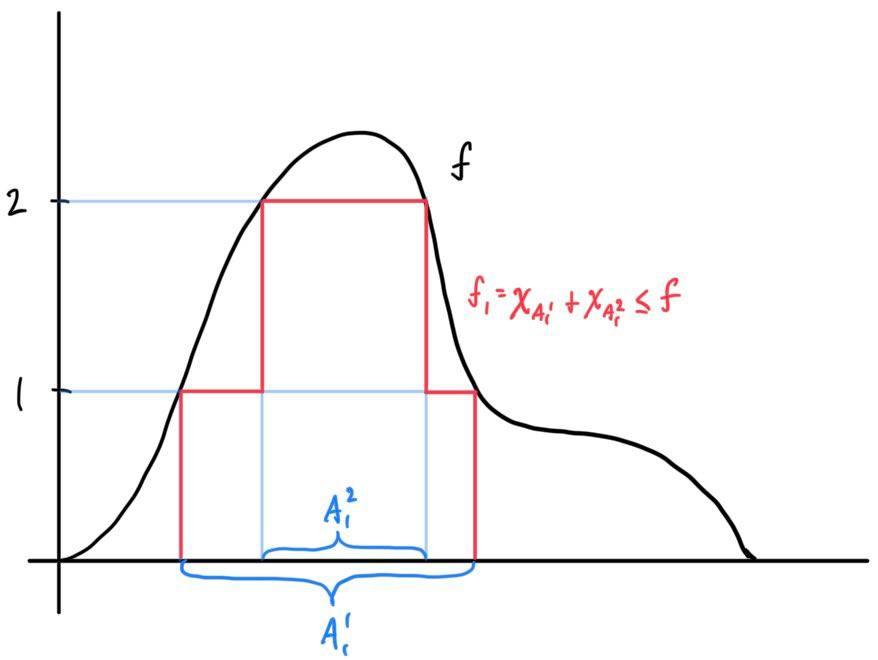
\includegraphics[scale=0.23]{img/simple_approximation_1.jpg}
        \caption{}
      \end{subfigure}
      \hfill 
      \begin{subfigure}[b]{0.48\textwidth}
        \centering
        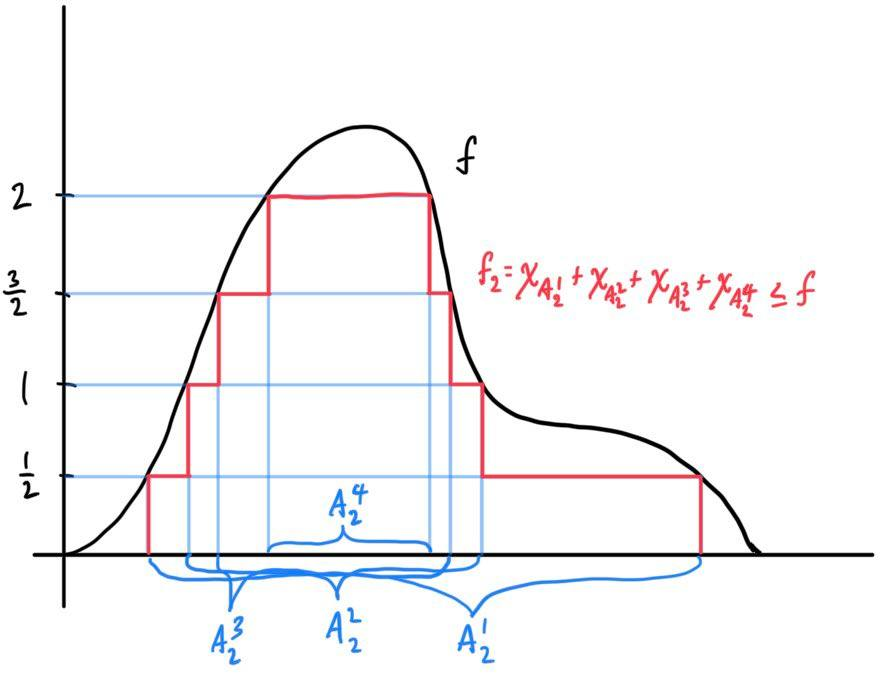
\includegraphics[scale=0.23]{img/simple_approximation_2.jpg}
        \caption{For the next partition, consider a smaller $\epsilon = \frac{1}{2}$. }
      \end{subfigure}
      \caption{}
    \end{figure}

    \begin{enumerate}
      \item $(\rightarrow)$. First, assume that $f \geq 0$. Then, for all $n \in \mathbb{N}$, define 
      \begin{equation}
        E_n \coloneqq \{ x \in E \mid f(x) \leq n \}
      \end{equation}
      Then, $E_n$ is a measurable set, and the restriction of $f$ to $E_n$ is a nonnegative bounded measurable function. Now we can invoke the simple approximation lemma on $f|_{E_n}$, but to make sure that the $\phi_n$'s actually converge, we should let the $\epsilon$ error also decrease to $0$---say $\epsilon = \frac{1}{n}$. So, we have 
      \begin{equation}
        0 \leq \phi_n \leq f \leq \psi_n, \quad 0 \leq \psi_n - \phi_n \leq \frac{1}{n}
      \end{equation}
      on $E_n$. Note that 
      \begin{equation}
        0 \leq \phi_n \leq f, \qquad 0 \leq f - \phi_n \leq \psi_n - \phi_n < \frac{1}{n} 
      \end{equation}
      Now, we escape $E_n$ and extend $\phi_n (n) = n$ if $f(x) > n$. Therefore, the function $\phi_n$ is simple and $\phi_n \leq f$ on all of $E$. We claim that $\phi_n \to f$. 
      \begin{enumerate}
        \item \textit{Case 1}. Let $f$ be finite. Then we can choose a natural $N \in \mathbb{N}$ s.t. $f(x) \leq N$. Then, 
        \begin{equation}
          n \geq N \implies 0 \leq f(x) - \phi_n (x) < \frac{1}{n} 
        \end{equation}
        and so $\lim_{n \to \infty} \phi_n (x) = f(x)$. 

        \item \textit{Case 2}. Assume $f(x) = +\infty$. Then, $\phi_n (x) = n$ for all $n$, so $\lim_{n \to \infty} \phi_n (x) = f(x)$. 
      \end{enumerate}
      By replacing each $\phi_n$ with $\max\{\phi_1, \ldots, \phi_n\}$, we have $(\phi_n)$ increasing. 

      \item $(\leftarrow)$. Since simple functions are measurable, $\phi_n \to f$ which is measurable, and we are done. 
    \end{enumerate}
  \end{proof}
  \begin{proof}
    We give a general picture of this proof for a function $f: \mathbb{R} \longrightarrow [0, \infty]$. We can first divide the codomain of the graph below into segments of $t = 1, 2, \ldots$, and take the preimage of all these units under $f$ to get $f_1$. More specifically, $A_1^t = f^{-1} ([t, \infty])$ for all $t$. By measurability of $f$, $A_1^t$ is measurable, and we can assign $f_1 = \chi_{A^1_1} + \chi_{A_1^2} \leq f$. 
    Doing this again with finer subintervals of the codomain gives us, with $f_2 = \chi_{A_2^1} + \chi_{A_2^2} + \chi_{A_2^3} + \chi_{A_2^4} \leq f$, and in general, we have $f_k = \sum_{j=1}^\infty \frac{1}{2^{k-1}} \chi_{A^j_k}$. But we said a simple function is a \textit{finite} sum, and if $\infty$ is in the range of $f$, then this becomes a problem. We can quickly fix this by just truncating the summation at a certain point in the codomain ($f_1$ only considers intervals up to $1$, $f_2$ up to $2$ and so on), ultimately giving us 
    \begin{equation}
      f_k = \sum_{j=1}^{k 2^{k-1}} \frac{1}{2^{k-1}} \chi_{A^j_k} 
    \end{equation}
  \end{proof}

\subsection{Nearly Uniform Convergence of Measurable Functions} 

  We have proved one of the first big theorems on measurable functions: that limit of measurable functions is also measurable. But we would like to find ways to extract \textit{uniform} convergence. This is where another major idea of measure theory---Littlewood's third principle---comes in.\footnote{The first principle was that every measurable set is nearly an open set. The second principle, ironically, will come last.} 


  The next proof requires a new technique that allows us to almost ``hack out'' uniform convergence. Let $f_n \to f$ pointwise on $E$. How can we make $f_n$ converge uniformly? The simplest way is to restrict the domain,\footnote{In the most extreme case, let us strict $E$ to a single point. Then, convergence is equivalent to uniform convergence.} and we can do this in three stages. Fix $\epsilon > 0$. 
  \begin{enumerate}
    \item \textit{Remove Dependency on $x$}. 
    For a fixed $x \in E$, we can see that there exists $N = N_x \in \mathbb{N}$ s.t. 
    \begin{equation}
      n \geq N_x \implies |f_n (x) - f(x)| < \epsilon
    \end{equation}
    This $N_x$ is dependent on $x$, but simply by focusing on the $x$'s that satisfy the above, we can consider 
    \begin{equation}
      E_N \coloneqq \{x \in E \mid |f_n (x) - f(x)| < \epsilon \; \forall n \geq N \}
    \end{equation}
    It's a little bit odd, but makes sense. Usually, we are given a fixed $x$ and then proceed to find a $N$. Now, we are working backwards: we take a fixed $N$ and look for all the $x$'s such that $f_n(x)$ lie close to $f(x)$ after $N$. By doing this, we manually remove the dependency on $x$. So, if $x \in E_N$, then we can literally pick the same index $N = N$ so that $|f_n (x) - f(x)| < \epsilon$ for $n \geq N$. 

    \item \textit{Add Flexibility to choose $N$}. This gets a bit closer to uniform convergence, but this is too restrictive since we can \textit{always} choose $N$ for $E_N$,\footnote{Say $N = 100$. Then, $x \in E_N$ implies that $|f_n (x) - f(x)| < \epsilon$ for $n \geq 100$, but it never says anything about whether $N$ can be $101$ or $1000$.} where in uniform convergence, we just need to find \textit{one} such $N$. Therefore, we can ``expand'' our restriction to 
    \begin{equation}
      A = \bigcup_{N = 1}^\infty E_N  \subset E
    \end{equation}
    Therefore, if $x \in A$, then $x \in E_N$ for some $N$, which means that there exists $N \in \mathbb{N}$ s.t. $|f_n (x) - f(x)| < \epsilon$ for all $n \geq N$. Boom. 

    \item \textit{Apply to all $\epsilon$}. Note that $A = A_\epsilon$ is really dependent on the $\epsilon$ that we have fixed so far. Now we must be able to choose for all $\epsilon > 0$. In order to do this, we must take the intersection 
    \begin{equation}
      \bigcap_{\epsilon > 0} A_\epsilon
    \end{equation}
    I think this is usually the most restrictive, and kills most of the set. 
  \end{enumerate}

  Note that the following Egorov's lemma just requires us to prove up to the second point, while Egorov's theorem will require us to prove to the third. 

  \begin{lemma}[Egorov]
    Let $(f_n: E \subset \mathbb{R} \to \mathbb{R})$ be a sequence of measurable functions with $m(E) < +\infty$ that converges pointwise to $f$. Then, for each $\eta > 0$ and $\delta > 0$, there exists a measurable subset $A \subset E$ and index $N$ such that 
    \begin{equation}
      |f_n - f| < \eta \text{ on } A \text{ for all } n \geq N, \text{ and } m(E \setminus A) < \delta 
    \end{equation}
  \end{lemma}
  \begin{proof}
    The general idea is to first use the manual hack to make $f_k \to f$ uniformly on a restricted domain. Second, we want to try and expand this domain as much as possible to cover $E$. 
    \begin{enumerate}
      \item Note that since $f_k \to f$ pointwise, $f$ is measurable, and since $x \mapsto |x|$ is continuous, the function $|f_k - f|$ is measurable. Therefore, we use the hack above and see that 
      \begin{align}
        E_K & \coloneqq \{ x \in E \mid |f_k (x) - f(x)| < \eta \; \forall k \geq K \} \\ 
            & = \bigcap_{k=K}^\infty \{x \in E \mid |f_k (x) - f(x)| < \eta \}
      \end{align}
      which is a countable collection of measurable sets and hence measurable. Great, so given $\eta > 0$, we can see that $f_k$ does not deviate from $f$ by more than $\eta$ \textit{globally} on $E_K$. 

      \item If we did not have the $m(E \setminus A) < \delta$ condition, we could stop here. However, we do, so we must try and expand $E_K$ somehow. Note that we can just union over $K$ to get $\cup_{K=1}^\infty E_K = E$ since $f_k \to f$ and see that 
      \begin{equation}
        m \bigg( \bigcup_{K=1}^\infty E_K \bigg) = m(E) < +\infty
      \end{equation}
      At this point, we might be tempted to call $A = E$ and call it a day. But note that in this case, the index $N$ that we are looking for is not fixed, since $x \in A \implies x \in E_K$ for some $K \in \mathbb{N}$, and so $N = K$. But notice that $E_K \subset E_{K+1}$, and so by continuity from below, 
      \begin{equation}
        \lim_{K \to \infty} m(E_K) = m(E) < +\infty
      \end{equation}
      Since it converges to a finite nmber, $\exists N \in \mathbb{N}$ s.t. 
      \begin{equation}
        m(E) - m(E_N) < \delta
      \end{equation}
      So setting $A = E_N$ and by excision property, we get $m(E \setminus E_N) < \delta$. 
    \end{enumerate}
  \end{proof}


  The next theorem is one we will use all the time. It basically tells us a way to turn a sequence of pointwise convergent functions into a sequence of uniformly convergent functions. It seems similar to \hyperref[real-thm:dini]{Dini's theorem} in that it gives conditions of uniform integrability for a sequence of pointwise convergence functions. 

  \begin{theorem}[Egorov]
    Let $(f_n: E \subset \mathbb{R} \to \mathbb{R})$ be a sequence of measurable functions with $m(E) < +\infty$ that converges pointwise to $f$. Then, for each $\epsilon > 0$, there exists a closed set $F \subset E$  s.t. 
    \begin{equation}
      f_n \to f \text{ uniformly on } F \text{ and } m(E \setminus F) < \epsilon
    \end{equation}
  \end{theorem}
  \begin{proof}
    Don't worry too much about the closed set. Most of the work has been done for us in the lemma, where we have completed the first 2 stages of conversion from pointwise to uniform convergence. We know that for \textit{fixed} $\eta, \delta > 0$, we can find a measurable set $A_\eta \subset E$ and index $N_\eta$ s.t. 
    \begin{equation}
      |f_n - f| < \eta \text{ on } A_\eta \text{ for all } n \geq N_\eta, \qquad m(E \setminus A) < \delta
    \end{equation}
    The main work is to remove the dependency of $A$ and $N$ on $\eta$ so that it works globally. 

    Fix $\epsilon > 0$. For each $n \in \mathbb{N}$, let $A_n \subset E$ and $N_n \in \mathbb{N}$ be such that 
    \begin{equation}
      |f_k - f| < \frac{1}{n} \text{ on } A_n \text{ for all } k \geq N_n, \qquad m(E \setminus A_n) < \frac{\epsilon}{2^{n+1}}
    \end{equation}
    We are basically constructing the $A_n$ so that it gradually fills up $E$ \textit{and} the errors $|f_k - f|$ are getting smaller, but at the cost of $N_n$ also increasing. Now define 
    \begin{equation}
      A = \bigcap_{n=1}^\infty A_n 
    \end{equation}
    And we can see that $A$ is within our tolerance 
    \begin{equation}
      m(E \setminus A) = m \bigg( \bigcup_{n=1}^\infty E \setminus A_n \bigg) \leq \sum_{n=1}^\infty m (E \setminus A_n) < \sum_{n=1}^\infty \frac{\epsilon}{2^{n+1}} = \frac{\epsilon}{2}
    \end{equation}
    We claim that $f_n \to f$ uniformly on $A$. Let $\epsilon > 0$, then choose index $n_0$ s.t. $\frac{1}{n_0} < \epsilon$. Then, 
    \begin{equation}
      k \geq N_{n_0} \implies |f_k - f| < \frac{1}{n_0} \text{ on } A_{n_0} 
    \end{equation}
    Since $A \subset A_0$ and $1/n_0 < \epsilon$, we have 
    \begin{equation}
      k \geq N_{n_0} \implies |f_k - f| < \epsilon \text{ on } A 
    \end{equation}
    Therefore $f_n \to f$ uniformly with $m(E \setminus A) < \frac{\epsilon}{2}$. Finally, for the closed part, since $A$ is measurable (as countable intersection of measurable sets), we just find some closed set $F \subset A$ s.t. $m(A \setminus F) < \frac{\epsilon}{2}$. 
  \end{proof}

\subsection{Continuous Approximations of Measurable Functions}

  Finally, we prove the results of Littlewood's second principle. That is, if we throw out a small set, we can approximate measurable functions with continuous functions. 

  \begin{lemma}[Luzin, for Simple Functions]
    Suppose $f: E \subset \mathbb{R} \to \mathbb{R}$ is simple. Then $\forall \epsilon > 0$, there exists 
    \begin{enumerate}
      \item a closed $F \subset E$, and 
      \item a continuous function $g: \mathbb{R} \to \mathbb{R}$
    \end{enumerate}
    such that
    \begin{equation}
      f = g \text{ on } F, \qquad m(E \setminus F) < \epsilon
    \end{equation}
  \end{lemma}
  \begin{proof}
    Let $a_1, \ldots, a_n$ be the finite number of distinct values taken by $f$ on the disjoint measurable sets $E_1, \ldots, E_n$. Take closed sets $F_1, \ldots, F_n$ s.t. 
    \begin{equation}
      F_k \subset E_k, \qquad m(E_k \setminus F_k) < \frac{\epsilon}{n}
    \end{equation}
    Then, $F = \cup_{k=1}^n F_k$ is closed and since $E_k$'s are disjoint, 
    \begin{equation}
      m(E \setminus F) = m \bigg( \bigcup_{k=1}^n (E_k \setminus F_k) \bigg) = \sum_{k=1}^n m(E_k \setminus F_k) < \epsilon
    \end{equation}
    Let $g = f$ on all $F_k$. Now it remains to establish continuity, which we can do with the Tietze extension theorem.\footnote{Or just order the closed sets and linearly interpolate between their endpoints(?)}
  \end{proof}

  \begin{theorem}[Luzin]
    Suppose $f: E \subset \mathbb{R} \to \mathbb{R}$ is measurable. Then $\forall \epsilon > 0$, there exists 
    \begin{enumerate}
      \item a closed $F \subset E$, and 
      \item a continuous function $g: \mathbb{R} \to \mathbb{R}$
    \end{enumerate}
    such that 
    \begin{equation}
      f = g \text{ on } F, \qquad m(E \setminus F) < \epsilon
    \end{equation}
  \end{theorem}
  \begin{proof}
    The general idea is to combine all the theorems we learned so far. First, we use the simple approximation theorem to find a sequence of simple functions that converge pointwise to $f$. Then, we branch off in two independent directions. On one hand, we use Egorov to establish uniform convergence, and on the other hand, we use Lusin's lemma to establish continuity. Finally, we combine the two with the result that uniform limits of continuous functions are continuous. 

    Assume $m(E) < \infty$. If it is $\infty$, then we can divide the set into countable sets, each with finite measure, and we can do it for $\epsilon/2^{n}$. So it suffices for finite measure. Let's start. 

    According to the simple approximation theorem, there is a sequence of simple functions $\phi_n \to f$ on $E$. Now we branch off. 
    \begin{enumerate}
      \item \textit{Establish Continuous Approximations}. Now for each $\phi_n$, we can apply Luzin's theorem for simple functions to find closed $F_n \subset E$ and continuous $g_n$ s.t. 
      \begin{equation}
        \phi_n = g_n \text{ on } F_n, \qquad m(E \setminus F_n) < \frac{\epsilon}{2^{n+1}} 
      \end{equation}

      \item \textit{Establish Uniform Convergence}. Use Egorov's theorem to find a closed set $F_0 \subset E$  s.t. $\phi_n \to f$ uniformly on $F_0$, with $m(E \setminus F_0) < \frac{\epsilon}{2}$. 
    \end{enumerate}
    Now we want to restrict the domain to a set that has both of these properties. Define 
    \begin{equation}
      F = \bigcap_{n=0}^\infty F_n
    \end{equation}
    which is closed. Also, each $\phi_n$ is continuous on $F$ since $F \subset F_n$ and $\phi_n = g_n$ on $F_n$, and $\phi_n \to f$ uniformly on $F \subset F_0$. Finally, 
    \begin{equation}
      m(E \setminus F) = m \bigg( [E \setminus F_0] \cup \bigcup_{n=1}^\infty [E \setminus F_n] \bigg) \leq \frac{\epsilon}{2} + \sum_{n=1}^\infty \frac{\epsilon}{2^{n+1}} = \epsilon
    \end{equation}
    Since the uniform limit of continuous functions is continuous, $f |_F$ is continuous on $f$, and we can use Tiezte extension theorem to extend this to all of $\mathbb{R}$. 
  \end{proof}
  \begin{proof}
    In class. Assume $m(E) < \infty$. If it is $\infty$, then we can divide the set into countable sets, each with finite measure, and we can do it for $\epsilon/2^{n}$. So it suffices for finite measure. Suppose $f_n$ are simple and $f_n \to f$ pointwise on $E$. By the lemma, we can find closed $F_n \subset E$ s.t. $m(E \setminus F_n) < \epsilon / 2^{n+1}$ and $g_n \in C(\mathbb{R})$, with $g_n |_{F_n} = f_n |_{F_n}$. Also, by Egorov, we can find $F_0$ s.t. $f_n$ converges uniformly on $F_0$, and $m(E \setminus F_0) < \epsilon / 2$. Define 
    \begin{equation}
      F = \bigcap_{n=0}^\infty F_n, \qquad E \setminus F = \bigcup_{n=0}^\infty E \setminus F_n
    \end{equation}
    Then by subadditivity,
    \begin{equation}
      m(E \setminus F) \leq \sum_{n=0}^\infty m(E \setminus F_n) < \epsilon
    \end{equation}
    Finally, $f_n$ converges uniformly on $F$ and $f_n |_F = g_n |_F$, so $f_n$ are continuous on $F$. Since uniform limit of continuous functions is continuous, the limit $f$ is continuous on $F$. 
  \end{proof}

  This is an argument for the interval, but this can be generalized to more general sets. 

